\documentclass[11pt]{article}
\usepackage{mgates-letter}
\definecolor{dark_blue} {rgb}{0., 0., 0.65}
\usepackage{makecell}
\usepackage[
backend=biber,
style=alphabetic,
%citestyle=numeric,
%entrykey=false,
%annotation=false,
url=false
]{biblatex}

\usepackage{textcomp}
\usepackage{mathrsfs}  % mathscr font
\usepackage{boxedminipage}
\usepackage{rotating}
\usepackage{csquotes}
%\usepackage{natbib}
\usepackage[colorlinks, filecolor=dark_blue, urlcolor=dark_blue, linkcolor=black, citecolor=black]{hyperref}

\defbibcheck{mine}{\iffieldequalstr{annotation}{mine}{}{\skipentry}}
\defbibcheck{other}{\iffieldequalstr{annotation}{other}{}{\skipentry}}

\addbibresource{biblio.bib}

\begin{document}
\sloppy
\begin{center}
	{{
		\Large{
			\textsc{PhD Programme in Computer Science and Engineering \\ 
			\vspace{4mm}
			Cycle XXXVI}
			}
	}} 
	\rule[0.1cm]{\textwidth}{0.1mm}
	\rule[0.4cm]{\textwidth}{0.6mm}
\end{center}

\begin{center}
	{\LARGE{A Language-based Software Engineering Approach for Cyber-Physical Swarms}} \\
	\vspace{4mm}
	{\large{PhD Year II -- Report}} 
	\vspace{4mm}
\end{center}
\vspace{8mm}
\par
\noindent
\begin{minipage}[t]{0.47\textwidth}

{\large{Commission: \\\bf
Prof. Mirko Viroli \\
Prof. Andrea Omicini \\
Prof. Matteo Ferrara} 
}
\end{minipage}
\hfill
\begin{minipage}[t]{0.47\textwidth}
	\raggedleft
	{
		\large{PhD Student: \\\bf Gianluca Aguzzi}
	}
\end{minipage}
\vspace{10mm}

{
	\raggedright
	\rule[0.1cm]{\textwidth}{0.6mm}
	\rule[0.5cm]{\textwidth}{0.1mm}
}

\newcommand{\rev}[1]{{
	%\color{red}
	#1
	}}
\section{Introduction}
In the last decades, several research topics, such as pervasive~\cite{pervasive}, 
 ubiquitous~\cite{weiser1999computer}, collective~\cite{abowd2016beyond}, everyware~\cite{greenfield2010everyware} computing, 
 foster a vision in which thousands of computational devices, 
 ranging from smartphones, personal computers, and embedded devices,
 collaborate which each other to build complex applications.
%
Given this context, in my research, I call these large-scale multi-agent systems \textit{Cyber-Physical Swarms} (CPSWs).
%
The name came from natural inspiration, since this large ensemble of computational devices, 
 from a global perspective, could be seen as a ``swarm'' of simple entities that, with complex interactions, 
 perform complicated collective tasks.
%
Moreover, the entities are \textit{cyber-physical} since they have an \textit{embodiment} in the environment, 
 namely, they have a physical counterpart with which they can sense and alter the physical world.
%
This vision embraces several kinds of systems, such as
 swarm robotics, ``swarms'' of people (crowds) or, in general, ``swarms'' of IoT devices.

Designing applications for CPSWs is demanding for several reasons, just to mention some:
 i) the environment in which entities belong is highly unpredictable,
 ii) the collective behaviour could have long unstable transient, and
 iii) there is no central authority that coordinates the agents. 
%
Nowadays, researchers are trying to handle these challenges by working 
 on the development of robust self-adaptive collective behaviour
 like the one observed in a natural environment --- so failure-resistant, efficient, and effective. 
%
Then, as main research goal of my PhD, I want to find a systematic methodology (models, techniques and algorithms) 
 to synthesise and deploy self-organising behaviours of predictable outcomes for CPSW.
%
In particular, I follow a language-based approach, where the models and tools are built around
 a target programming language.
%
In my research, 
 I mainly leverage Aggregate Computing (AC)~\cite{beal2015aggregate} ---a novel top-down global-to-local programming model. 
%
I choose this language since the abstractions that it exposes, 
 make the development of collective application in the CPSWs scenario easier:
 the entire collective behaviour is seen as an evolution of \textit{computational fields},
 that could be manipulated with a functional and declarative approach.
%
Even if AC is already applied in several use cases, 
 there is a need to both explore new research directions and
 to improve the current state-of-the-art solutions in order to close the reality gap, 
 making it possible to use AC in modern distributed applications.
%
In this second year then, 
 I make works in this direction, 
 both exploring new distributed algorithms and devising the research area 
 --- i.e., integrating Reinforcement Learning (RL) with AC framework. 

\section{Activities}
\begin{figure}
	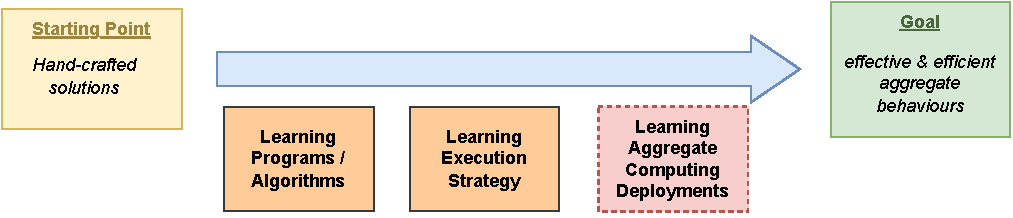
\includegraphics[width=\textwidth]{roadmap.pdf}
	\caption{
		Overview of the activities carried out for the integration of learning with AC. 
		The orange blocks are the one that was explored during this year. 
		The red block (i.e., learning deployment) is the one that I will explore in my last year.
	}
	\label{fig:overview}
\end{figure}
This year, 
 I was mainly focused on integrating Machine Learning techniques into the Aggregate Computing stack.
%
This integration has several benefits, 
 including improving the adaptivity of aggregate systems, 
 and separating functional specifications (i.e., aggregate code) from non-functional ones (e.g., consumption, convergence times, ...).
%
As a first work, in \textit{\citefield{roadmap}{title}} I have drafted 
 a roadmap in which I discuss possible directions in which 
 aggregate computing and machine learning can be combined. 
%
In the article, I present the main directions of this integration (Figure 1), which are:
\begin{itemize}
	\item Learning aggregate programs/algorithms: designing efficient and versatile AC algorithms can be complex, 
	therefore, it is interesting to explore whether algorithms can be learnt or synthesised given high-level functional goals.
	
	\item Learning execution strategy: for a given AC program or algorithm, 
	 multiple execution strategies can be applied, 
	 affecting aspects like the scheduling
	 of computation rounds, 
	 the scheduling of communications, 
	 the retention of messages from neighbours. 
	%
	Novel approaches~\cite{zambonelli2021time} 
	 adapt the execution choices at runtime 
	 depending on factors which may include the speed of environmental change, 
	 the energy level of a device, incentives in volunteering settings, 
	 or the desired Quality of Service.
	Since it is hard to design static
	 or dynamic execution strategies able 
	 to adequately take into account all the factors and goals, 
	 it could be possible to let a system (and its components) 
	 learn how to efficiently execute algorithms according 
	 to a set of given high-level objectives.
	
	\item Learning aggregate computing deployments: a logical AC system consists of a logical network of
	 logical devices operating following a specified execution protocol. 
	As shown in recent work on pulverised architectures~\cite{Casadei2020}, 
	 it turns out that different application partitioning schemas and implementations of the digital thread associated 
	 with the aggregate system are possible, 
	 as well as different deployments of application components onto the available Information-Communication Technology (ICT) infrastructure. 
	In this context, ML could be injected to have 
	 the system learns by itself what is a (locally) optimal deployment 
	 for an aggregate application.
\end{itemize}
Till now, I have focused mainly on improving 
 the definition of aggregate programs with reinforcement learning 
 and enhancing collective scheduling policies.
%
Concerning the integration of learning in aggregate programming, the work 
 entitled \textit{\citefield{aguzzi2022towards}{title}} 
 discusses the use of RL as a way to learn pieces of code 
 that may be sensitive to environmental conditions. 
In this work, we were inspired by program sketching 
 and we use a version of Q-learning~\cite{watkins1992q} for multi-agent systems (Hysteric Q-Learning~\cite{matignon2007hysteretic})
 to handle the complex interaction between the nodes. 
 
In \textit{\citefield{rl-middleware}{title}} instead, 
 we used RL to learn scheduling policies 
 in order to optimize consumption 
 while maintaining good responsiveness w.r.t. the collective behaviour.  
This work can be seen as an extension of the one \textit{\citefield{zambonelli2021time}{title}} 
 in which AC itself is used to define scheduling policies. 
With our approach, it is possible 
 to learn online the policy that can 
 maximize energy savings while maintaining low consumption.

In parallel to these works related to the combination of AC and RL, 
 I have also explored the development of algorithms/patterns/methodologies 
 that can be applied in the context of CPWs.
%
In the \textit{\citefield{swarm-clustering}{title}} 
 we explored a new clustering technique to track space-time evolving phenomena. 
% 
These clusters can then be used at the application level to perform 
 distributed decision-making and/or create related cluster-wise synthesise information.
Our approach, unlike standard approaches found in literature, 
 works in a distributed and iterative manner by exploiting 
 aggregate processes -- abstraction introduced in Aggregate Computing 
 that allows concurrent collective computations.

\textit{\citefield{domains}{title}} considers a design abstraction used to
 devise complex decentralized computation in complex collective ecosystems.
%
The main abstraction, called \textit{dynamic decentralization domains}, is used to
 create a region in space that opportunistically will be formed to support distributed 
 sensing and acting.
%
In the paper, we also show the implementation of that abstraction using Scala.

For what concern the engineering methodologies, in \textit{\cite{engineering}{title}}
 we examine the issues of engineering aggregate systems, outlining then a research roadmap that exemplifies
 how the automation and methodological approach could improve the current
 trial-and-error approach.
%
Finally, in \textit{\citefield{scafi-paper}{title}}, we describe ScaFi, 
 a toolkit used for Aggregate Computing written in Scala.
ScaFi is not new, in fact I am one of the main contributors to the software and I am the lead designer of
 ScaFi Web~\cite{aguzzi2021scafi} --- A playground used to try Aggregate Computing online.
We made this article then, to make ScaFi more accessible to a broad scientific community, 
 since, currently, it is still not vastly applied in the community of collective systems.

\subsection{Period Abroad}
In August, I started my period abroad 
 at Aarhus University under the supervision of Lukas Esterle.
%
During this period, I was mainly interested in applying Graph Neural Networks (GNNs)~\cite{scarselli2008graph}
 -- A neural network that works on graphs -- 
 with Aggregate Computing programs.
%
In particular, I used GNN to forecast 
 the state of natural phenomena tracked by agents of an aggregate system, and then, 
 using Aggregate Programming, we would like to coordinate the agent in a way 
 that they could follow the phenomena of interest.
%
In doing this, we applied a Centralised Training and Decentralised Execution (CTDE)~\cite{foerster2018deep} approach. 
%
In this way, the learning local features using global data, 
 and then we can ``break'' the neural architecture in each node of the system.
%
This could be done since GNN can be also understood as a local application of matrix multiplication.
%
This integration has a broader impact on the research of Aggregate Computing combined with Machine Learning. 
%
Indeed, this could be used in the work already 
 explore to extract a representation of the local state agent 
 --- that, in fact, we found particularly hard using hand-craft solutions. 

\section{Talks}
\begin{enumerate}
	\item Towards Reinforcement Learning-based Aggregate Computing @ COORDINATION 2022
	\item Machine Learning for Aggregate Computing: a Research Roadmap @ DISCOLI 2022
	\item Addressing Collective Computations Efficiency: Towards a Platform-level Reinforcement Learning Approach @ ACSOS 2022
\end{enumerate}
\section{International Conference Activities}
\begin{enumerate}
	\item Artifact Evaluation Committee @ COORDINATION 2022
	\item Student Volunteer @ ICDCS 2022
	\item Student Volunteer @ ACSOS 2022
	\item Sub-reviewer @ COORDINATION 2022
	\item Sub-reviewer @ AAMAS 2022
	\item Sub-reviewer @ DISCOLI 2022
	\item Sub-reviewer @ ASE NIER 2022
\end{enumerate}
\section{Teaching}
\begin{enumerate}
	\item Tutor @ Padigmi di Progettazione e Sviluppo (PPS)
	\item Tutor @ Programmazione Concorrente e Distribuita (PCD)
	\item Seminar entitled ``Scala: a Cross-Platform Language'' @ PPS
	\item Seminar entitled ``Scala(e) to the large. Concurrent programming in Scala and relevant Frameworks'' @ PPS
	\item Seminar entitled ``Akka: An introduction'' @ PCD
	\item Seminar entitled ``Akka for Distributed Systems'' @ PCD
\end{enumerate}
\section{Courses and School}

\begin{table}[H]
	\resizebox{\textwidth}{!}{%
	\begin{tabular}{|c|c|c|c|c|c|}
	\hline
		Professor & Course & Kind & Credits & Period & Exam \\ \hline
		Enrico Gallinucci & From Big Data to Data Platform & PhD Course & \makecell{10 hours \\ 2 proposed credits} & \makecell{January \\ 2022} & Not done \\ \hline
		Roberto Casadei & \makecell{Engeneering Collective Intelligence} & PhD Course & \makecell{10 hours \\ 2 proposed credits} & \makecell{December \\ 2020} & Done \\ \hline
		Marco Gori & \makecell{Towards Developmental Machine Learning} & \makecell{BISS 2022 \\ Spring School} & \makecell{10 hours \\ 4 credits } & \makecell{April \\ 2022} & Done \\ \hline
		Massimo Villari & \makecell{From Cloud to Serverless through microelements} & \makecell{BISS 2022 \\ Spring School} & \makecell{10 hours \\ 4 credits } & \makecell{April \\ 2022} & Done \\ \hline
		Armir Bujari & \makecell{Industry 4.0 and the Industrial Internet of Things: \\ Challenges and Enabling Technologies} & \makecell{PhD Course} & \makecell{15 hours \\ 3 credits } & \makecell{February \\ 2022} & Done \\ \hline
		Aristides Gionis & \makecell{Opinions and conflict in social networks: \\ models, computational problems, and algorithms} & \makecell{BISS 2022 \\ Spring School} & \makecell{X} & \makecell{February \\ 2022} & Not Done \\ \hline
		X & \makecell{MOOC \\ Introduction to Complexity \\ \href{https://www.complexityexplorer.org/courses/119-introduction-to-complexity-2021}{\textbf{MOOC}}} & \makecell{MOOC} & \makecell{15 hours \\ 3 proposed credits} & \makecell{September \\ 2022} & \makecell{Done} \\ \hline
	
	\end{tabular}
	}
\end{table}

\section{Papers}
\subsection{Published}
\begin{itemize}
	\item \fullcite{swarm-clustering}
	\\{\footnotesize\textbf{Abstract:} \citefield{swarm-clustering}{abstract}}
	\item \fullcite{aguzzi2022towards}
	\\{\footnotesize\textbf{Abstract:} \citefield{aguzzi2022towards}{abstract}}
\end{itemize}
\subsection{Accepted}
\begin{itemize}
	\item \fullcite{scafi-paper}
	\\{\footnotesize\textbf{Abstract:} \citefield{scafi-paper}{abstract}}
	\item \fullcite{roadmap}
	\\{\footnotesize\textbf{Abstract:} \citefield{roadmap}{abstract}}
	\item \fullcite{engineering}
	\\{\footnotesize\textbf{Abstract:} \citefield{engineering}{abstract}}
	\item \fullcite{rl-middleware}
	\\{\footnotesize\textbf{Abstract:} \citefield{rl-middleware}{abstract}}
\end{itemize}
\subsection{In Peer Review}
\begin{itemize}
	\item \fullcite{domains}
	\\{\footnotesize\textbf{Abstract:} \citefield{domains}{abstract}}
\end{itemize}
\section{References}
\printbibliography[heading=none, check=other]

\end{document}
